\documentclass[10pt]{article}
\usepackage[margin=0.85in]{geometry}
\usepackage{amsmath,amssymb,bm}
\usepackage{booktabs}
\usepackage{graphicx}
\usepackage{enumitem}
\usepackage{xurl}
\usepackage[hidelinks]{hyperref}
\usepackage{caption}
\usepackage{subcaption}
\usepackage{titlesec}
\usepackage{xcolor}
\usepackage{tikz}
\usetikzlibrary{arrows.meta,calc}
\titlespacing*{\section}{0pt}{10pt}{4pt}
\titlespacing*{\subsection}{0pt}{8pt}{3pt}
\captionsetup{font=small,labelfont=bf,skip=4pt}
\setlist{itemsep=2pt,topsep=3pt,leftmargin=1.4em}
\setlength{\parskip}{2pt}
\newcommand{\Tr}{\mathrm{Tr}}
\newcommand{\bQ}{Q^\dagger}
\definecolor{nodeA}{HTML}{0072B2}
\definecolor{nodeB}{HTML}{D55E00}
\definecolor{nodeC}{HTML}{009E73}
\title{\vspace{-1.5cm}\Large\textbf{The Fermionic $U(n)^3$ Quiver: BPS Entropy, Concentration, and Chaos}\\[2pt]
\normalsize Progress report, October 2026\vspace{-6pt}}
\author{}
\date{}

\begin{document}
\maketitle
\vspace{-1.0cm}
\begin{center}\begin{minipage}{0.95\textwidth}\small
\textbf{Abstract.} We study a purely fermionic, $\mathcal N=2$ supersymmetric gauged quantum mechanics that, as far
as we can tell, has not been considered before: three bifundamental fermions $A$, $B$, $C$ of $U(n)^3$ arranged on
a triangle quiver, each in $p$ flavours, with the cubic supercharge $Q=\sum C_{abc}\Tr(A^aB^bC^c)$. It is the matrix
($D=2$) member of the coloured models of Gurau--Witten type, so its large-$n$ limit is planar, and it was chosen
because bifundamental matter has no zero weights, which removes the mechanism that makes the BPS window of adjoint
matrix models grow with the rank. In the gauge-singlet sector, exact cohomology at $(n,p)=(2,2)$ and Lanczos
diagonalisation at $(2,3)$ show that all singlet BPS states, 90 and 1680 of them, sit at half filling, and all 90
classes at $(2,2)$ are fortuitous. At $p=3$ the singlet multiplet spectrum has
Gaussian-orthogonal level statistics over $10\,024$ levels and small gaps only next to the BPS degree, while $p=2$
turns out to be special, with a hidden $\mathcal N=4$ supersymmetry on singlets and a spectrum that is not
random-matrix like. We then show that the singlet index is exactly the partition function of a three-species log
gas on the circle. This proves $I_0(n,2)=(-1)^n(3n)!/(n!)^3$ and fixes the sign of the index in general, and the
large-$n$ saddle gives $\ln|I_0|=F^*(p)\,n^2+O(\ln n)$ with $F^*>0$ exactly when $p>2$; at $p=3$,
$F^*=1.2373$, which is $41\%$ of the singlet log-count, and as $p\to\infty$ the BPS entropy per fermion approaches
the $\mathcal N=2$ SYK value $\frac12\ln3$. A parameter-free finite-$n$ evaluation of the same saddle reproduces all
27 non-zero exact indices and singlet counts to within $0.6$ in the logarithm. The $p\ge3$ quiver therefore has
macroscopic BPS entropy, concentration and chaos at the sizes we can reach; concentration at $n\ge3$, fortuity at
$p\ge3$ and genuine near-BPS scaling are the open questions, and we describe how to attack them.
\end{minipage}\end{center}
\vspace{8pt}

\section{Introduction}\label{sec:intro}

The fortuity programme proposes that the BPS states responsible for the entropy of supersymmetric black holes are
cohomology classes that exist at a given rank but cannot be continued to larger rank, as opposed to monotone
classes that are inherited along a tower of ranks \cite{ChangLin}. Chang, Chen, Sia and Yang argued that a theory
whose BPS states are mostly fortuitous should exhibit R-charge concentration \cite{CCSY}: within each complex, the
BPS states sit in a single degree of the R-charge. $\mathcal N=2$ SYK is the paradigm \cite{FGMS}. There the BPS
states occupy a window of width $\hat q$ around half filling, their number grows exponentially with the number of
fermions, and the non-BPS spectrum next to them is chaotic, with the density of states of the $\mathcal N=2$
super-Schwarzian \cite{TW}. Chen asked for the simplest \emph{matrix} model with these properties, a ``matrix SYK''
model: purely fermionic matrix quantum mechanics with a cubic supercharge built from traces \cite{Chen}. He showed
that a single adjoint fermion already has fortuitous BPS states, although they spread over $N+1$ charges, and
suggested that three adjoint flavours might concentrate.

Our earlier reports \cite{R1,R2} analysed this adjoint family in detail and reached a negative conclusion. At the
maximal weight the BPS window has width $W=r(w_s-1)+1$ for a gauge algebra of rank $r$, where the width $w_s\ge2$
contributed by a single Cartan site is controlled by one bilinear form. The window therefore grows with the rank,
and a concentrated large-$N$ limit is impossible for adjoint matter at fixed degree of the supercharge. The
mechanism lives on the Cartan: the adjoint representation has zero weights, and at the maximal weight the complex
is a product of Cartan sites, each of which contributes its own spread in charge. This points to an obvious way
out, namely to build the cubic supercharge from matter without zero weights. The simplest such matter is
bifundamental, and the simplest cubic gauge invariant of bifundamentals is the trace around a triangle,
$\Tr(ABC)$.

This report collects what we have learned about the resulting model. We describe it in Section~\ref{sec:model} and
place it in the literature in Section~\ref{sec:lit}. Section~\ref{sec:bps} presents the exact and numerical results
on BPS states at small rank: singlet indices, concentration at $(n,p)=(2,2)$ and $(2,3)$, and a fortuity test.
Section~\ref{sec:spectrum} turns to the non-BPS singlet spectrum, where $p=3$ is chaotic and $p=2$ has a hidden
extended supersymmetry. Section~\ref{sec:largen} contains the main analytic result: the singlet index is the
partition function of a three-species log gas, which we solve at large $n$. Section~\ref{sec:prospects} assesses
the prospects of the $p\ge3$ model and lists the next steps.

\section{The model}\label{sec:model}

The gauge group is $U(n)_0\times U(n)_1\times U(n)_2$, with fundamental indices $i$, $j$ and $l$ for the three
nodes. The matter consists of complex fermions
\begin{equation}
A^a_{ij}\in(\mathbf n,\bar{\mathbf n},\mathbf 1),\qquad B^a_{jl}\in(\mathbf 1,\mathbf n,\bar{\mathbf n}),\qquad
C^a_{li}\in(\bar{\mathbf n},\mathbf 1,\mathbf n),\qquad a=1,\dots,p,
\end{equation}
transforming as $A\to g_0Ag_1^{-1}$, $B\to g_1Bg_2^{-1}$ and $C\to g_2Cg_0^{-1}$, with canonical anticommutators
such as $\{A^a_{ij},(A^b_{i'j'})^\dagger\}=\delta^{ab}\delta_{ii'}\delta_{jj'}$. We regard $A$, $B$ and $C$ as
creation operators acting on a Fock vacuum annihilated by their adjoints. The Hilbert space is the exterior algebra
$\mathcal H=\Lambda^\bullet V$ on the $3pn^2$ modes of $V=\mathbb C^p\otimes\big[(\mathbf n,\bar{\mathbf n},\mathbf
1)\oplus(\mathbf 1,\mathbf n,\bar{\mathbf n})\oplus(\bar{\mathbf n},\mathbf 1,\mathbf n)\big]$, of dimension
$2^{3pn^2}$. The dynamics is fixed by a single supercharge,
\begin{equation}
Q=\sum_{a,b,c=1}^pC_{abc}\,\Tr\big(A^aB^bC^c\big)=\sum_{a,b,c}C_{abc}\,A^a_{ij}B^b_{jl}C^c_{li},\qquad
H=\{Q,\bQ\}\ge0 .
\label{eq:Q}
\end{equation}
Because $Q$ is a product of three creation operators it acts on $\mathcal H$ as exterior multiplication by a fixed
gauge-invariant three-form, and $Q^2=0$ holds identically: no condition is imposed on the couplings, which form an
arbitrary tensor $C\in\mathbb C^p\otimes\mathbb C^p\otimes\mathbb C^p$. (The three fields are distinct, so no
symmetrisation is implied, and flavour rotations $U(p)^3$ act on $C$.) All numerical results below use generic
couplings, mostly random integers between 1 and 5 with a fixed seed, and several Gaussian real and complex sets as
checks. Figure~\ref{fig:quiver} shows the quiver and the interaction vertex.

\begin{figure}[t]\centering
\begin{subfigure}[b]{0.46\textwidth}\centering
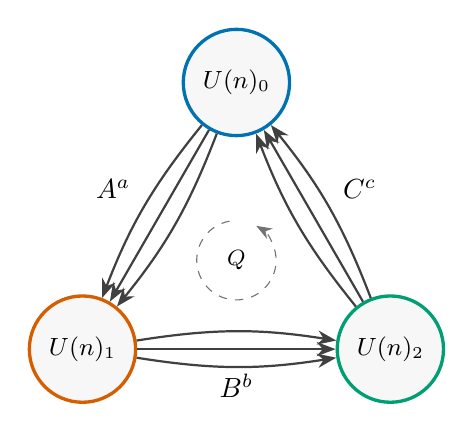
\begin{tikzpicture}[scale=1.05,
  qnode/.style={circle,draw,very thick,minimum size=1.35cm,fill=gray!6,font=\small},
  arr/.style={-{Stealth[length=2.4mm,width=1.8mm]},thick,black!75}]
  \node[qnode,draw=nodeA] (n0) at (90:2.15) {$U(n)_0$};
  \node[qnode,draw=nodeB] (n1) at (210:2.15) {$U(n)_1$};
  \node[qnode,draw=nodeC] (n2) at (330:2.15) {$U(n)_2$};
  \foreach \b in {-9,0,9} {
    \draw[arr] (n0) to[bend left=\b] (n1);
    \draw[arr] (n1) to[bend left=\b] (n2);
    \draw[arr] (n2) to[bend left=\b] (n0);
  }
  \node at (150:1.72) {$A^a$};
  \node at (270:1.52) {$B^b$};
  \node at (30:1.72) {$C^c$};
  \draw[-{Stealth[length=2mm]},dashed,black!55] (0,0) ++(100:0.48) arc (100:420:0.48);
  \node[font=\footnotesize] at (0,0) {$Q$};
\end{tikzpicture}
\caption{}\label{fig:quiver-a}
\end{subfigure}\hfill
\begin{subfigure}[b]{0.46\textwidth}\centering
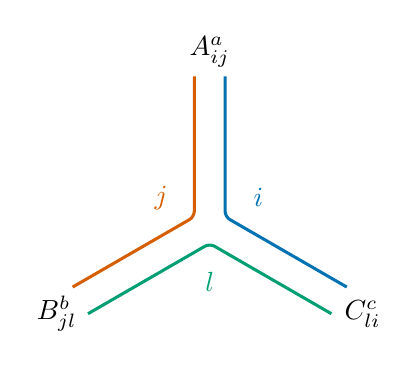
\begin{tikzpicture}[scale=1.15,line width=1.1pt]
  \def\dd{0.17}
  \def\rr{1.65}
  \draw[nodeB,rounded corners=2pt] ($(90:\rr)+(180:\dd)$) -- (150:1.155*\dd) -- ($(210:\rr)+(120:\dd)$);
  \draw[nodeC,rounded corners=2pt] ($(210:\rr)+(300:\dd)$) -- (270:1.155*\dd) -- ($(330:\rr)+(240:\dd)$);
  \draw[nodeA,rounded corners=2pt] ($(330:\rr)+(60:\dd)$) -- (30:1.155*\dd) -- ($(90:\rr)+(0:\dd)$);
  \node at (90:1.92) {$A^a_{ij}$};
  \node at (210:1.95) {$B^b_{jl}$};
  \node at (330:1.95) {$C^c_{li}$};
  \node[nodeA] at (30:0.62) {$i$};
  \node[nodeB] at (150:0.62) {$j$};
  \node[nodeC] at (270:0.62) {$l$};
\end{tikzpicture}
\caption{}\label{fig:quiver-b}
\end{subfigure}
\caption{(a) The quiver. An arrow from node $v$ to node $v+1$ (mod 3) is a bundle of $p$ fermionic bifundamentals
in $(\mathbf n_v,\bar{\mathbf n}_{v+1})$, drawn here for $p=3$. The supercharge \eqref{eq:Q} is the gauge-invariant
loop around the triangle, with a general flavour tensor $C_{abc}$. (b) The interaction as a ribbon vertex. Each
field carries the indices of the two nodes it joins, and each index line closes around the vertex. This is the
$D=2$ member of the coloured models of \cite{Witten}; at large $n$ only planar ribbon graphs survive.}
\label{fig:quiver}
\end{figure}

The theory has a $U(1)^3$ of fermion numbers $N_A$, $N_B$, $N_C$, each raised by one unit by $Q$. Two combinations
of them, $N_A-N_C$ and $N_B-N_A$, are the central charges of the gauge nodes, so gauge singlets have
$N_A=N_B=N_C=m$ and total fermion number $k=N_A+N_B+N_C=3m$. The total fermion number plays the role of the
R-charge, and $Q$ raises it by $\hat q=3$. BPS states, $H\psi=0$, are in one-to-one correspondence with $Q$-cohomology
classes, and we write $h^k$ for their number in degree $k$ and $n(k)$ for the number of gauge singlets in degree
$k$. The pairing with the top form of $\Lambda^\bullet V$ exchanges $k$ and $3pn^2-k$, so $n(k)$ is palindromic and
$h^k=h^{3pn^2-k}$, and half filling is $k_*=3pn^2/2$. Non-BPS states come in $Q$-pairs $(\psi,Q\psi)$ in degrees $k$
and $k+3$ with a common energy, and we label the pair by its charge relative to half filling,
$q=k+\tfrac32-\tfrac32pn^2$, following \cite{TW}. Since $(-1)^k$ anticommutes with $Q$, the singlet index
\begin{equation}
I_0(n,p)=\sum_m(-1)^m\,n(3m)=\sum_m(-1)^m\,h^{3m}_{\rm sing}
\label{eq:index}
\end{equation}
is a lower bound on the number of singlet BPS states. The bound is saturated when the singlet BPS states sit in a
single degree, which is what concentration means here. In $\mathcal N=2$ SYK with $\hat q=3$ the BPS states fill
three adjacent charges in the ratio $1{:}2{:}1$ \cite{FGMS,TW}; gauge singlets live only in degrees $k\equiv0$ mod
3, so for even $pn^2$ that window contains exactly one singlet degree, half filling, and concentration of the
singlet sector means that every singlet BPS state has $k=3pn^2/2$. By Molien--Weyl, $n(t)=\sum_kn(k)t^k$ is the
unitary matrix integral
\begin{equation}
n(t)=\int\prod_{v=0}^2dU_v\;\prod_{v=0}^{2}\det\big(1+t\,U_v\otimes U_{v+1}^\dagger\big)^p,\qquad I_0=n(-1),
\label{eq:MW}
\end{equation}
over Haar measure, with $v$ taken mod 3. This integral is the starting point of Section~\ref{sec:largen}.

Two structural remarks explain why the model was chosen and where its interesting range of parameters lies. The
weights of the bifundamental modes are differences $e_i-f_j$ of weights of two different nodes and never vanish,
so the zero-weight (Cartan) modes on which the window-widening mechanism of the adjoint models lives are simply
absent. This removes the obstruction of \cite{R1,R2}; it does not by itself imply concentration. Second, the gauge
group has dimension $3n^2$ against $3pn^2$ fermion modes, a ratio of $p$ rather than a large number, so the
singlet constraint is severe. At $p=1$ it leaves essentially nothing: at $n=2$ and $3$ every irrep's complex has
index $\pm1$, the singlet index vanishes, and concentration is vacuous. The model becomes interesting at $p\ge2$.

\section{Relation to previous work}\label{sec:lit}

Witten obtained the large-$N$ physics of SYK without disorder from a coloured model of $q=D+1$ fermion fields of
rank $D$, every pair of which shares one index \cite{Witten}. For $q=3$ and $D=2$ the three fields are exactly
bifundamentals of a three-node quiver and the vertex is $\Tr(ABC)$. Witten's melonic dominance argument, however,
requires $D\ge3$ (his eq.~(3.10)); at $D=2$ the relevant combinatorial invariant reduces to the genus of ribbon
graphs and the large-$n$ limit is planar. Our model is the complex, flavoured, $\mathcal N=2$ supersymmetric version
of this matrix member of the coloured family. Supersymmetric tensor versions of SYK exist with $\mathcal N=1$ supersymmetry and
higher-rank tensors \cite{PSV}. Chang, Colin-Ellerin and Rangamani showed that $\mathcal N=2$ supertensor models with
dynamical bosons break supersymmetry at large $N$, and noted that the purely fermionic $\mathcal N=2$ model with
an odd-degree supercharge has no evident melonic tensor version (their eq.~(6.4)) \cite{CCR}. Biggs, Lin and
Maldacena have since closed that gap melonically, replacing tensor contractions by $SU(2)$ $3j$ symbols
\cite{BLM}. The quiver is a planar counterpart: purely fermionic, cubic and $\mathcal N=2$, without dynamical
bosons and hence without the supersymmetry-breaking mechanism of \cite{CCR}.

The same three-node quiver with a closed loop and a cyclic cubic superpotential is famous in a different guise, as
the quiver quantum mechanics of three-centre BPS bound states in string theory. For bosonic chiral multiplets on
abelian nodes, Bena, Berkooz, de Boer, El-Showk and Van den Bleeken found exponentially many ``pure-Higgs'' states
that are invisible on the Coulomb branch and are natural candidates for single-centre black hole microstates
\cite{Bena}; they also remarked that their counting formula suggests an origin in fermionic degrees of freedom.
Our model is a different theory, purely fermionic and non-abelian, whose BPS states are the cohomology of a finite
Fock space with no Higgs or Coulomb branch, and we claim no equivalence; a naive comparison of our $n=1$ counts with
theirs already fails.

On the fortuity side, the monotone/fortuitous dichotomy and the covering construction are due to Chang and Lin
\cite{ChangLin}, and concentration as its signature in SYK to \cite{CCSY}. Chen constructed fortuitous states in a
single adjoint matrix and used a unitary matrix integral to follow them as the rank changes \cite{Chen}. Tierz
computed BPS spectra of $\Tr\Psi^p$ models and formulated fortuity through projections between ranks, which are
cochain maps \cite{Tierz}; we use his definition. Choi, Choi and Kim studied fortuity in the bifundamental conifold
theory and introduced ``generalised monotones'' dressed by baryons \cite{CCK}, which bears directly on our fortuity
test (Section~\ref{sec:fortuity}). The natural tool for large $n$ is the quantum mechanical matrix bootstrap
\cite{HHK,LZ,LM}, which Chen already suggested for matrix SYK models; our sector-resolved version is described in
\cite{R2}. A literature search in October 2026 found no previous study of the fermionic quiver itself, although
absence from searches is not proof.

\section{BPS states at small rank}\label{sec:bps}

\subsection{Singlet indices}

The singlet multiplicities $n(k)$ follow from the dual Cauchy identity,
$\Lambda(\mathbb C^p\otimes V_v\otimes\bar V_{v+1})=\bigotimes_{f=1}^p\bigoplus_\lambda S_\lambda V_v\otimes
S_{\lambda'}\bar V_{v+1}$, which reduces the singlet count to products of Littlewood--Richardson coefficients. We
compute these by exact quadrature on the torus and assemble the index with a transfer matrix over $U(n)$ irreps
that adds one flavour at a time,
\begin{equation}
I_0=\Tr\big[(R^{(p)})^3\big],\qquad R^{(q)}=\sum_\lambda(-1)^{|\lambda|}\,L_\lambda^{\,T}R^{(q-1)}L_{\lambda^T},\qquad
(L_\lambda)_{\mu\nu}=c^\nu_{\mu\lambda},
\end{equation}
in exact integer arithmetic. This reaches $(n,p)=(4,3)$ and $(3,4)$ and reproduces every value obtained earlier by
direct weight counting. Table~\ref{tab:index} lists the results together with the total singlet counts.

\begin{table}[t]\centering\small
\begin{tabular}{cccrcc}
\toprule
$(n,p)$ & modes $3pn^2$ & singlet states & $I_0(n,p)$ & $\ln|I_0|$ per mode & $(-1)^{pn^2/2}$ \\
\midrule
$(1,2)$ & 6 & $10$ & $-6$ & 0.299 & $-$\\
$(2,2)$ & 24 & $1\,274$ & $90$ & 0.187 & $+$\\
$(3,2)$ & 54 & $2\,115\,632$ & $-1\,680$ & 0.138 & $-$\\
$(4,2)$ & 96 & $5.59\times10^{10}$ & $34\,650$ & 0.109 & $+$\\
\midrule
$(1,3)$ & 9 & $56$ & $0$ & -- & ($pn^2$ odd)\\
$(2,3)$ & 36 & $889\,040$ & $1\,680$ & 0.206 & $+$\\
$(3,3)$ & 81 & $4.90\times10^{12}$ & $0$ & -- & ($pn^2$ odd)\\
$(4,3)$ & 144 & $1.08\times10^{22}$ & $9\,434\,197\,872$ & 0.159 & $+$\\
\midrule
$(1,4)$ & 12 & $346$ & $90$ & 0.375 & $+$\\
$(2,4)$ & 48 & $9.70\times10^{8}$ & $519\,750$ & 0.274 & $+$\\
$(3,4)$ & 108 & $2.99\times10^{19}$ & $199\,090\,719\,360$ & 0.241 & $+$\\
\midrule
$(1,5)$ & 15 & $2\,252$ & $0$ & -- & ($pn^2$ odd)\\
$(2,5)$ & 60 & $1.37\times10^{12}$ & $95\,866\,056$ & 0.306 & $+$\\
$(1,6)$ & 18 & $15\,184$ & $-1\,680$ & 0.413 & $-$\\
$(2,6)$ & 72 & $2.29\times10^{15}$ & $28\,686\,212\,100$ & 0.334 & $+$\\
\bottomrule
\end{tabular}
\caption{Exact gauge-singlet indices and singlet counts. The $n=1$ rows are Dixon's sum
$\sum_m(-1)^m\binom pm^3$ and the Franel numbers $\sum_m\binom pm^3$. At $p=1$ the index vanishes for $n=2,3,4$. The
last column is the sign that a singlet BPS sector concentrated at half filling would give; it agrees with every
non-zero entry.}
\label{tab:index}
\end{table}

Three features of the table are worth stating at once. First, the $p=2$ entries are $(-1)^n(3n)!/(n!)^3$, a
formula that we found numerically and prove in Section~\ref{sec:largen}. The first few indices at $p=3$ coincided
with this pattern, $|I_0(2,3)|=|I_0(3,2)|=1680$, which briefly suggested that the index depends only on $np$ and
grows only exponentially in $n$; the value at $(4,3)$, which is about 550 times larger than the $p=2$-type value,
shows that the coincidence was accidental. Second, whenever $pn^2$ is even the sign of $I_0$ is $(-1)^{pn^2/2}$,
which is what a singlet BPS sector concentrated at half filling would produce, since half filling has
$m=pn^2/2$; for odd $pn^2$ the index vanishes identically, because the particle--hole map $m\to pn^2-m$ pairs
degrees of opposite sign. Third, at fixed $n$ the index per mode rises with $p$ towards the singlet entropy per
mode, which already suggests that large $p$ is the SYK-like direction.

\subsection{\texorpdfstring{Concentration at $(2,2)$ and $(2,3)$}{Concentration at (2,2) and (2,3)}}

At $(n,p)=(2,2)$ the singlet cohomology can be computed with exact (modular) ranks. There are exactly 90 singlet
BPS states, all at $k=12$, which is half filling, so the index is saturated. At $(2,3)$ the Fock space has $2^{36}$
states and the singlet sector at half filling has $300\,584$, which calls for a different method. We restrict to the
zero-weight subspace of each degree, which contains every irrep, and to the vectors invariant under the Weyl group
$(S_2)^3$, which commutes with $Q$ and fixes singlets; this reduces the dimension by about a factor of eight. On these
vectors the operator
\begin{equation}
P=\sum_{v=0}^2\big\|E^{(v)}_{12}\psi\big\|^2=\sum_v\langle\psi|J_v^2|\psi\rangle
\end{equation}
is the sum of the $SU(2)$ Casimirs of the three nodes, because $J_-J_+=J^2$ at $J_z=0$. It commutes with $H$,
vanishes exactly on singlets and is at least 2 on every non-singlet. The kernel of $K=H+\mu P$ is therefore the
singlet BPS space, and every eigenvalue of $K$ below $2\mu$ is an exact singlet energy. Lanczos diagonalisation of
$K$ in the degrees $k=9$, 12 and 15 (Weyl-symmetric dimensions $5.6\times10^4$, $5.1\times10^5$ and $1.8\times10^6$),
and dense diagonalisation for $k\le6$, finds no zero modes, with lowest eigenvalues $96.5$, $0.3348$ and $0.05386$
at $k=9$, 12 and 15; reruns at $k=12$ and 15 with different starting vectors reproduce them to nine digits. Particle--hole symmetry
excludes BPS states at $k\ge21$ as well, so all singlet BPS states sit at $k=18$, and by the index there are exactly
$h^{18}_{\rm sing}=|I_0|=1680$ of them. Figure~\ref{fig:concentration} summarises both cases: the singlet sector
spreads over 13 degrees at $(2,3)$, but its BPS states occupy one.

\begin{figure}[t]\centering
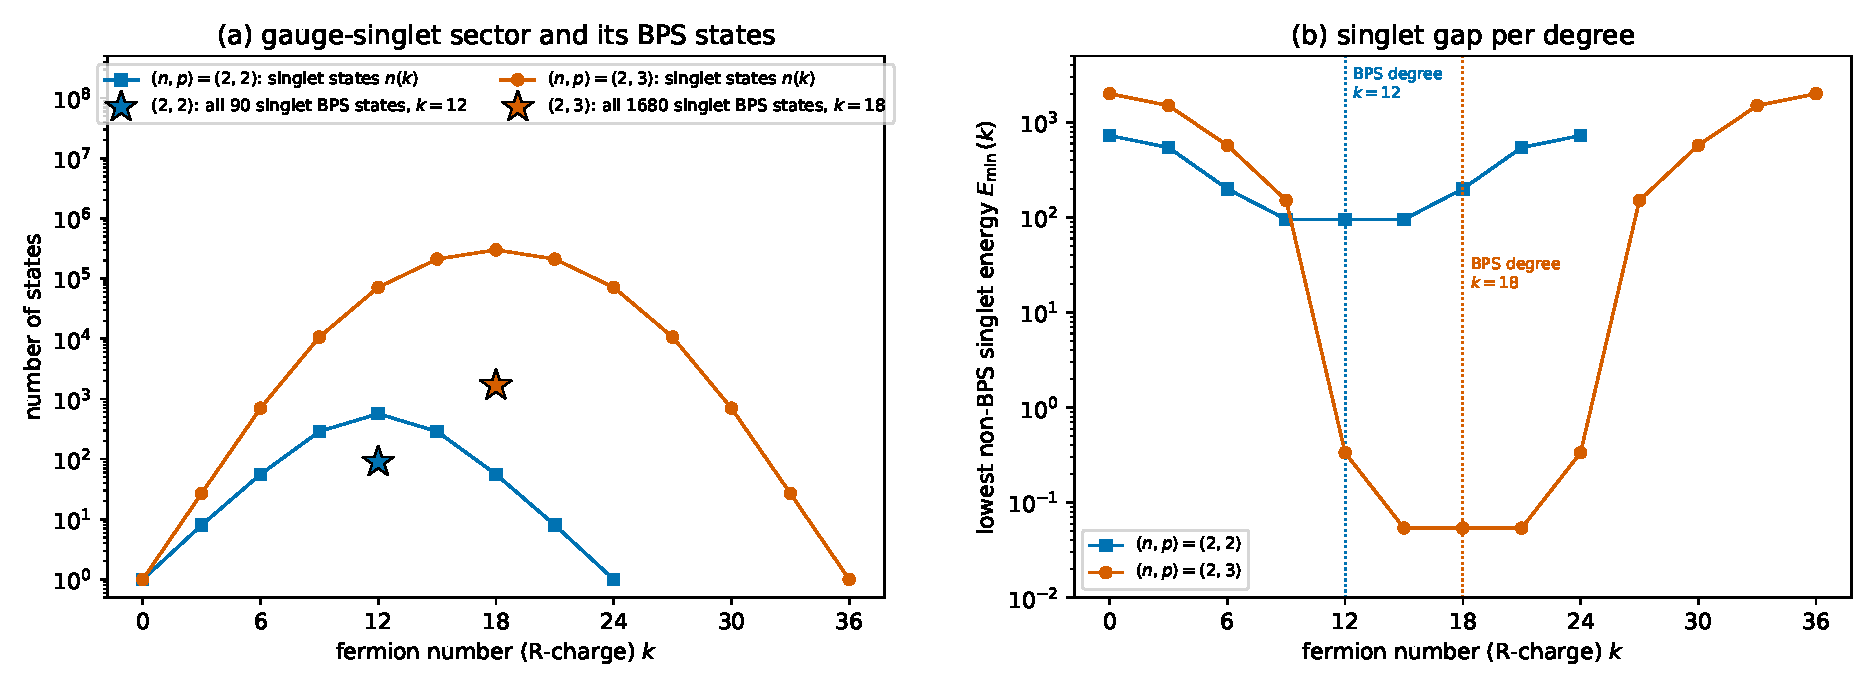
\includegraphics[width=0.98\textwidth]{report_figs/quiver_concentration.pdf}
\caption{Concentration of the singlet BPS states at $n=2$. (a) The number of gauge singlets in each degree $k$
(lines) and the singlet BPS states (stars): 90 at $k=12$ for $p=2$ (exact ranks) and 1680 at $k=18$ for $p=3$
(Lanczos); there are none in any other degree. (b) The lowest non-BPS singlet energy in each degree. At $p=3$ the
gap collapses by four orders of magnitude next to the BPS degree, to $0.054$ at $k=15,18,21$ and $0.335$ at
$k=12,24$, while at $p=2$ it never falls below $95.6$.}
\label{fig:concentration}
\end{figure}

A direct test at $n=3$ is out of reach for now. At $(3,2)$ the zero-weight sectors near half filling hold
$5\times10^{10}$ states, although the singlet subspaces are only about $5\times10^5$; what is missing is a cheap
explicit basis of singlets. The index there, $I_0(3,2)=-1680$, has the sign that concentration at half filling
($k=27$, $m=9$) would give, which is consistent with concentration but not evidence for it.

\subsection{\texorpdfstring{Fortuity at $(2,2)$}{Fortuity at (2,2)}}\label{sec:fortuity}

Following Tierz \cite{Tierz}, we call a rank-2 class monotone only if it lies in the image of the projection
$\pi_{3\to2}$ that deletes every monomial involving a third index on any node. Because $Q$ contains only creation
operators, $\pi Q^{(3)}=Q^{(2)}\pi$, so the projection is a cochain map. Writing $Q^{(3)}=Q^{(2)}+Q_{\rm new}$, a
closed rank-2 state $z_0$ is the projection of a closed rank-3 state if and only if $Q_{\rm new}z_0$ is exact in the
subspace of states that carry index-3 modes. Grading that subspace by the number of index-3 modes, the first
condition arises with two such modes, and for couplings of full rank in the summed flavour index it reduces to the
vanishing of the BPS three-point function $\langle\beta|X|z_0\rangle$ for every single letter $X$ and every BPS
state $\beta$ in degree $k+1$. A non-vanishing value obstructs the lift. By gauge covariance it suffices to test one
component of each letter. At $(2,2)$, each of the six letters obstructs a 54-dimensional subspace of the 90 classes,
different letters obstruct different subspaces, and together they obstruct all 90. Since the obstruction appears
already at the first order of the lift, none of the 90 classes lies in the image of $\pi_{3\to2}$: every singlet BPS
class at $(2,2)$ is fortuitous.

This result is expected rather than discriminating, and the reason can be made precise. The projections preserve
the degree, while the half-filling degree $k_*=3pn^2/2$ moves by $3p(2n+1)/2$ when the rank grows by one, more than
the width of any concentrated window. A rank-$n$ class of degree $k_*(n)$ can only be monotone if there is a class of
the same degree at rank $n+1$, so concentration at rank $n+1$ implies that every singlet BPS class at rank $n$ is
fortuitous; in this sense fortuity follows from concentration, much as in Chang--Chen--Sia--Yang's argument for
generic SYK \cite{CCSY}. At $(2,2)\to(3,2)$ the relevant rank-3 singlet space, at $k=12$, has only $3\,494$ states,
so the statement can be checked directly. The $(2,2)$ test itself uses one coupling and floating-point ranks, and it
is in the ordinary sense. Under the refined criterion of \cite{CCK},
classes of the form (determinant ground state)$\times$($n$-independent excitation) would count as generalised
monotones; with fermionic letters many determinants vanish, and whether any of the 90 classes is of that form has
not been analysed.

\section{\texorpdfstring{The singlet spectrum: chaos at $p=3$, hidden supersymmetry at $p=2$}{The singlet spectrum: chaos at p=3, hidden supersymmetry at p=2}}\label{sec:spectrum}

The exactness of the Casimir penalty makes the full singlet spectrum accessible at $n=2$. Where the singlet
subspace is small we construct it explicitly as $\ker P$ and diagonalise $(QU_k)^T(QU_k)$ on a singlet basis $U_k$,
whose non-zero eigenvalues are the multiplet energies of the pair $(k,k+3)$. For the largest pair at $(2,3)$,
$(9,12)$ with $10\,700$ singlets in the lower degree, we project random vectors onto singlets with the exact
polynomial $\prod_v\prod_{j=1}^{6}\big(1-J_v^2/j(j+1)\big)$, which leaves a non-singlet residual of
$1.4\times10^{-15}$, and compress $Q^TQ$ onto their span. Every count checks: the rank of the projected vectors equals
$n(9)$, the kernel equals the rank of the previous map, and the lowest level, $151.34$, agrees with Lanczos.

At $p=3$ the multiplet spectra are chaotic. The mean ratio of consecutive level spacings over the central $80\%$
of the $10\,024$ multiplets of the pair $(9,12)$ is $\langle r\rangle=0.5268\pm0.0028$. The Gaussian-orthogonal value
for matrices of the same size is $0.5343\pm0.0026$ and the Poisson value $0.3869\pm0.0042$, so the spectrum is about
30 standard deviations from Poisson and within two of the orthogonal class. The smaller pair $(6,9)$, with 676
levels, gives $0.507\pm0.011$, and the locally unfolded spacing distribution follows the Wigner surmise
(Figure~\ref{fig:step1}c). The orthogonal class is the expected one, since for real couplings $H$ is a real matrix in
the occupation-number basis.

The near-BPS structure is equally clear. The lowest multiplet energies of the pairs at $(2,3)$ are $0.05386$ for
$|q|=1.5$, the pairs adjacent to the BPS degree, then $0.3348$ for $|q|=4.5$, and then a jump to the microscopic
scale set by the couplings: $151.34$, $575.23$, $1506$ and $2008$ for $|q|=7.5$, $10.5$, $13.5$ and $16.5$.
Small gaps exist, and only next to the BPS degree (Figure~\ref{fig:concentration}b). A quantitative test of the
Turiaci--Witten density \cite{TW}, $\rho_q(E)\propto\sinh\big(2\pi\sqrt{(E-E_0(q))/E_s}\big)/E$ with
$E_0(q)=q^2E_s/4\hat q^2$, does not succeed at this size. Fixing $E_s=0.862$ from the $|q|=1.5$ edge predicts
$E_0=0.485$ at $|q|=4.5$, against $0.335$ measured, an edge ratio of $6.2$ instead of $9$; fixing the normalisation
from the eleven lowest $|q|=1.5$ levels predicts 5.4, 258, 2000 and $8.7\times10^4$ multiplets with $|q|=4.5$ below
$E=1.0$, $2.17$, $3.11$ and $5.38$, against 2, 3, 5 and 7 measured (Figure~\ref{fig:step1}d). This is not
surprising. The Turiaci--Witten density is a statement at large $e^{S_0}$ in which neighbouring charge sectors carry
the same entropy, whereas at $(2,3)$ the singlet sectors at $k=12$, 15 and 18 hold $71\,685$, $211\,113$ and $300\,584$
states, changing by factors of three to four per step. The test needs larger $n$.

The case $p=2$ behaves very differently, and the reason is an unexpected symmetry. The $(2,2)$ spectra are full of
exact coincidences between different pairs, and a search over cubic supercharges $\tilde Q=Q(\tilde C)$ that
commute with $H$ on singlets finds exactly one besides $Q$, namely
$\tilde C=(\varepsilon\otimes\varepsilon\otimes\varepsilon)\bar C$ with $\varepsilon$ the $2\times2$ antisymmetric
tensor. On every singlet sector, to $10^{-15}$, and for integer, Gaussian real and Gaussian complex couplings,
\begin{equation}
\tilde Q^2=0,\qquad\{Q,\tilde Q\}=0,\qquad\{Q^\dagger,\tilde Q\}=0,\qquad\{\tilde Q,\tilde Q^\dagger\}=H,
\end{equation}
which is an $\mathcal N=4$ algebra. Off the singlets the last two relations fail by about $30\%$ of $|H|$, so the
extended supersymmetry is a property of the gauged model, closing only up to gauge transformations. The singlet
spectrum organises completely into long $\mathcal N=4$ multiplets spanning degrees $k$, $k+3$, $k+3$ and $k+6$, with
$n(k)=b(k)+2b(k-3)+b(k-6)+h(k)$ in every degree. Once the flavour symmetry $F=\varepsilon$ on every edge (or the
corresponding antiunitary symmetry for complex couplings) is resolved, the level statistics are still not
random-matrix like in any symmetry class, with coupling-independent exact degeneracies, and within the span of all
gauge-invariant operators with at most four fermions the commutant of $H$ on the $k=9$ singlets is just $\{1,H\}$. At $p=3$ the
same search finds only $Q$. The hidden supersymmetry is plausibly tied to the pseudoreality of the $SU(2)$ flavour
doublet, but we have not derived it, and we have checked it only at $n=2$.

\begin{figure}[t]\centering
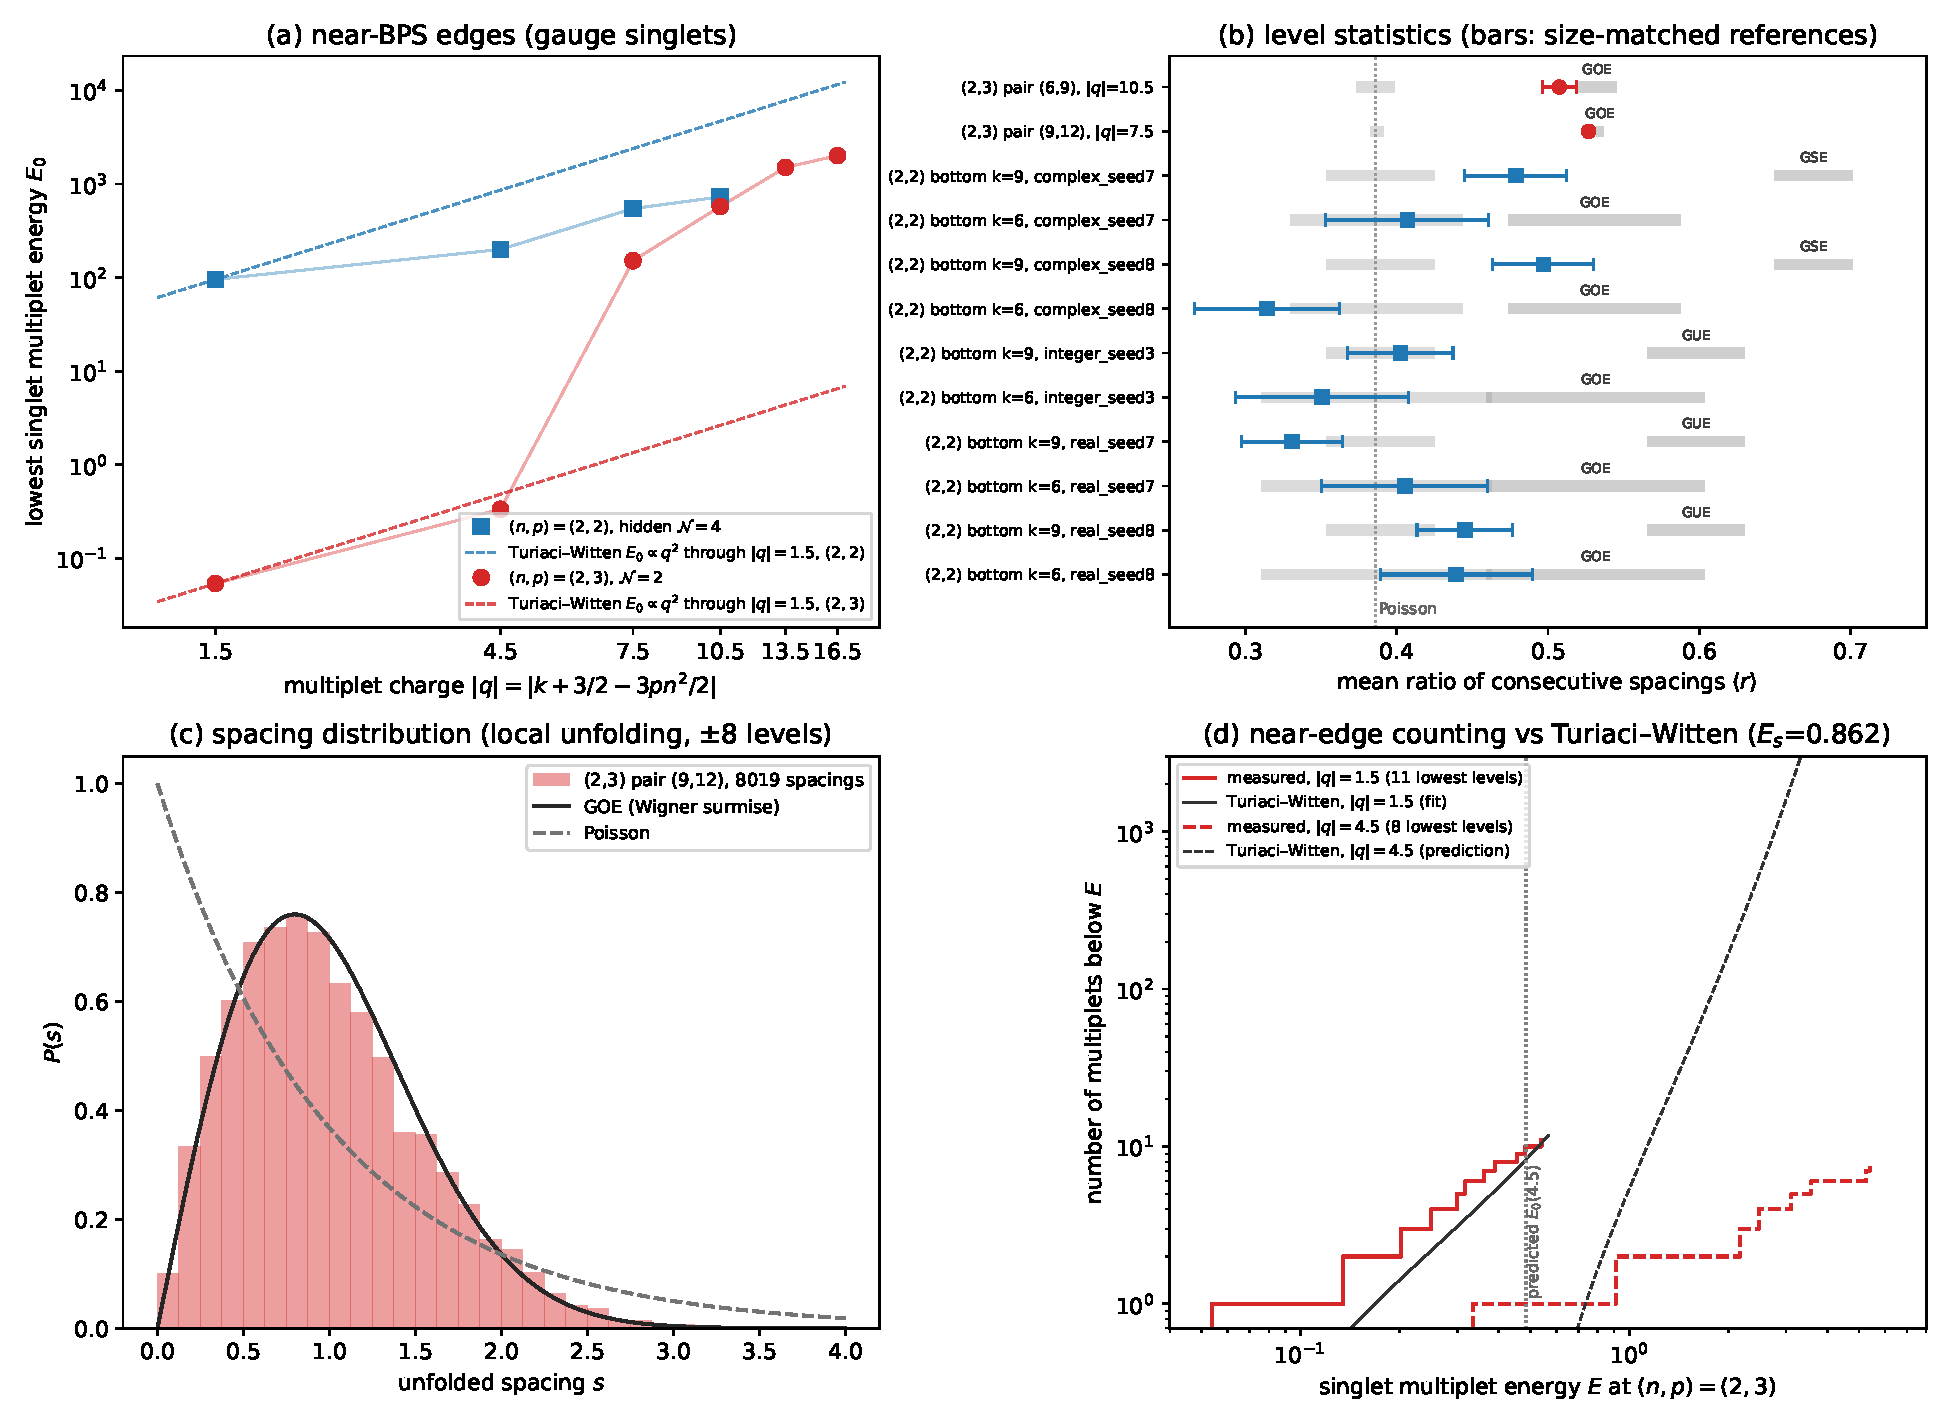
\includegraphics[width=0.98\textwidth]{report_figs/quiver_step1.pdf}
\caption{Singlet spectra at $n=2$. (a) Lowest singlet multiplet energy of each $Q$-pair against its charge $|q|$,
with the Turiaci--Witten $q^2$ law drawn through the $|q|=1.5$ point. (b) Mean spacing ratios of every
symmetry-resolved ensemble, with size-matched random-matrix and Poisson references. (c) Spacing distribution of the
$10\,024$ multiplets of the pair $(9,12)$ at $(2,3)$, locally unfolded, against the Wigner surmise and Poisson. (d)
Counting functions of the two innermost multiplet sectors at $(2,3)$ against the Turiaci--Witten density, normalised
on $|q|=1.5$; the $|q|=4.5$ curve is a prediction.}
\label{fig:step1}
\end{figure}

\section{\texorpdfstring{Large $n$: the singlet index as a three-species log gas}{Large n: the singlet index as a three-species log gas}}\label{sec:largen}

\subsection{An exact rewriting}

Write $x_{vi}=e^{i\theta_{vi}}$ for the eigenvalues of $U_v$ in \eqref{eq:MW} at $t=-1$. Weyl's integration
formula introduces $|\Delta(x_v)|^2/n!$ for each node, and the edge factors become
$\prod_{ij}\big(1-e^{i(\theta_{vi}-\theta_{v+1,j})}\big)^p$. For real $\varphi$,
$1-e^{i\varphi}=2\sin(\varphi/2)\,e^{i(\varphi-\pi)/2}$, and the $\varphi$-dependent phases cancel around the
triangle, since each node is the source of one edge and the target of another. Using
$|x_a-x_b|=|2\sin\frac{\theta_a-\theta_b}2|$,
\begin{equation}
\begin{gathered}
I_0(n,p)=\frac{(-i)^{3pn^2}}{(n!)^3}\int\prod_{v,i}\frac{d\theta_{vi}}{2\pi}\;e^{L(\theta)}\,\sigma(\theta)^p,\\
L=\sum_{\substack{\text{pairs at}\\\text{the same node}}}2\ln\big|2\sin\tfrac{\theta_a-\theta_b}2\big|
+p\!\!\sum_{\substack{\text{pairs at}\\\text{different nodes}}}\!\!\ln\big|2\sin\tfrac{\theta_a-\theta_b}2\big|,
\end{gathered}
\label{eq:loggas}
\end{equation}
with $\sigma=\prod_v\prod_{ij}\mathrm{sgn}\,\sin\frac{\theta_{vi}-\theta_{v+1,j}}2$. This is the partition function of
a gas of $3n$ charges of three species on the circle: charges of the same species repel with weight 2 and charges of
different species with weight $p$, and for odd $p$ there is an additional sign. Because every pair of distinct nodes
is joined by exactly one edge, $e^L$ is symmetric under permutations of the species, and only $\sigma$ remembers the
orientation of the quiver. The singlet count is the same integral with $|2\cos\frac{\theta_a-\theta_b}2|$ for pairs
at different nodes, which attract, and no phase.

Several exact statements follow immediately. At $p=2$ every pair carries weight 2 and $\sigma^2=1$, so $e^L$ is the
Vandermonde $|\Delta_{3n}(x)|^2$ of all $3n$ eigenvalues together. Its integral is $(3n)!$, and
\begin{equation}
I_0(n,2)=(-1)^n\frac{(3n)!}{(n!)^3}\qquad\text{for every }n .
\label{eq:p2}
\end{equation}
As measured by the index, the singlet BPS entropy of the $p=2$ model is therefore $3n\ln3+O(\ln n)$, which is not
macroscopic. The same manipulation, using $(1-x\bar y)^2=-x\bar y|x-y|^2$ on the unit circle, gives for general
$p$
\begin{equation}
I_0(n,p)=(-1)^n\frac{(3n)!}{(n!)^3}\;\mathbb E_{\mathrm{CUE}(3n)}\Big[\prod_v\prod_{i,j}\big(1-x_{vi}\bar x_{v+1,j}\big)^{p-2}\Big],
\end{equation}
where the $3n$ eigenvalues of a Haar-random $U(3n)$ matrix are split into three labelled groups. For even $p$ the
integrand of \eqref{eq:loggas} is positive, so $I_0\ne0$ with sign $(-i)^{3pn^2}=(-1)^{pn/2}$; for odd $p$ and odd $n$
the prefactor is $\pm i$ while the integral is real, so $I_0=0$; and for odd $p$, Cauchy--Schwarz in $p$ gives
$|I_0(n,p)|^2\le|I_0(n,p-1)|\,|I_0(n,p+1)|$, which holds in the data with ratios 16.6 at $(2,3)$ and 1.62 at $(2,5)$.
These are exactly the sign rules observed in Table~\ref{tab:index}.

\subsection{The saddle point}

At large $n$, with normalised eigenvalue densities $\rho_v$, $L=n^2F[\rho]+O(n\ln n)$ with
\begin{equation}
F[\rho]=\sum_v\langle\rho_v,f\rho_v\rangle+p\sum_{v<w}\langle\rho_v,f\rho_w\rangle,\qquad
f(\alpha)=\ln\big|2\sin\tfrac\alpha2\big|=-\sum_{m\ge1}\frac{\cos m\alpha}{m},
\end{equation}
and since $(n!)^3=e^{O(n\ln n)}$, $\ln|I_0|=n^2\max F+o(n^2)$ for even $p$ by standard log-gas large deviations. In
terms of the moments $u_{v,m}=\int\rho_v\,e^{im\theta}$, $F=-\sum_m\frac1m u_m^\dagger\big[\mathbb 1+\frac p2(J-\mathbb
1)\big]u_m$ with $J$ the all-ones $3\times3$ matrix, whose eigenvalues are $1+p$ for the species-symmetric
combination and $1-p/2$ twice. For $p<2$ the uniform distribution is a stable maximum with $F=0$; at $p=2$ it is
marginal; for $p>2$ it is unstable towards configurations in which the species separate, in the spirit of the
Hagedorn instability of weakly coupled gauge theories \cite{AMMPV}. The maximum then sits on the boundary of the
positivity constraint: the eigenvalues of the three nodes occupy three disjoint arcs rotated by $2\pi/3$ with
respect to each other (Figure~\ref{fig:saddle}d). Physically the holonomies sit near $U_v\approx e^{2\pi iv/3}$,
which turns the factor $(-1)$ that each bifundamental fermion carries in the index into a phase
$e^{\mp2\pi i/3}$ and so evades the cancellations between even and odd states that keep the index small at
$p\le2$.

We solve the continuum problem by expanding the density of one arc in Chebyshev polynomials. The Cauchy part of the
Euler--Lagrange equation is treated exactly and the smooth part by quadrature; the arc width follows from the
condition that the edges be soft, and $F^*$ is three times the Lagrange multiplier. The solution converges to twelve
digits, and the effective potential is flat on the support to $10^{-15}$ and lower in the gaps. Independently, Newton
maximisation of the discrete $L$ up to $n=2048$ extrapolates to the same coefficients to $10^{-9}$ or better, and for
$n\le12$ no unconstrained random start finds a higher maximum than the symmetric one. The singlet count is treated in
the same way: there the three species coincide on a single arc. Table~\ref{tab:saddle} gives the coefficients.

\begin{table}[t]\centering\small
\begin{tabular}{ccccccc}
\toprule
$p$ & $F^*$ (index) & arc half-width & $G^*$ (singlets) & $F^*/G^*$ & $F^*/3p$ & $G^*/3p$\\
\midrule
2 & 0 (exact) & $\pi/3$ & 1.4244 & 0 & 0 & 0.237\\
3 & 1.2373 & 1.0276 & 3.0427 & 0.41 & 0.137 & 0.338\\
4 & 2.5550 & 0.9717 & 4.7688 & 0.54 & 0.213 & 0.397\\
5 & 3.9297 & 0.9132 & 6.5623 & 0.60 & 0.262 & 0.437\\
6 & 5.3455 & 0.8606 & 8.4015 & 0.64 & 0.297 & 0.467\\
8 & 8.2619 & 0.7747 & 12.1714 & 0.68 & 0.344 & 0.507\\
16 & 20.4849 & 0.5796 & 27.8331 & 0.74 & 0.427 & 0.580\\
$\infty$ & $\frac{3p}2\ln3-\frac32\ln\frac{2p}3-\frac94$ & $\sqrt{6/p}$ & $3p\ln2-\frac32\ln\frac p2-\frac94$ &
$\frac{\ln3}{2\ln2}$ & $\frac12\ln3$ & $\ln2$\\
\bottomrule
\end{tabular}
\caption{Leading large-$n$ coefficients, $\ln|I_0|=F^*n^2$ and $\ln(\#\text{singlets})=G^*n^2$ up to $o(n^2)$, from
the continuum solution, with the large-$p$ asymptotics in the last row. The last two columns are per fermion mode.}
\label{tab:saddle}
\end{table}

Both limits can be derived analytically and are reproduced by the numerics. Near $p=2$ the uniform arcs of length
$2\pi/3$ give the bound $F^*(p)\ge(p/2-1)\,39\zeta(3)/2\pi^2$, which is tight as $p\to2^+$. At large $p$ the arcs
shrink to width $O(p^{-1/2})$, each becomes a semicircle of radius $\sqrt{6/p}$ in the effective harmonic potential of
the other two, and $F^*=\frac{3p}2\ln3-\frac32\ln\frac{2p}3-\frac94+O(1/p)$; the singlet count behaves in the same way
with $\ln2$ in place of $\frac12\ln3$. The leading terms have a simple meaning. $3p\ln2\,n^2$ is the logarithm of the
dimension of the whole Fock space, and $\frac{3p}2\ln3\,n^2$ is what $3pn^2$ fermion modes contribute when each
carries the weight $|1-e^{-2\pi i/3}|=\sqrt3$. The BPS entropy per fermion therefore approaches
$\ln\big(2\cos\frac\pi6\big)=\frac12\ln3$, which is precisely the ground-state entropy per complex fermion of
$\mathcal N=2$ SYK with $\hat q=3$ \cite{FGMS}, and the ratio $F^*/G^*$ approaches the SYK ratio
$\ln\sqrt3/\ln2=0.79$. The same constant appears in Tierz's large-$N$ result for the irrep-summed indices of the
single-matrix $\Tr\Psi^3$ model \cite{Tierz}. At finite $p$ the gauge constraint costs
$\frac1{2p}\ln\frac{2p}3+\frac3{4p}$ per mode, which is large at $p=3$: there the singlet BPS entropy per mode is
$0.137$, a quarter of the SYK value, but it is a finite fraction, $41\%$, of the singlet log-count.

\begin{figure}[t]\centering
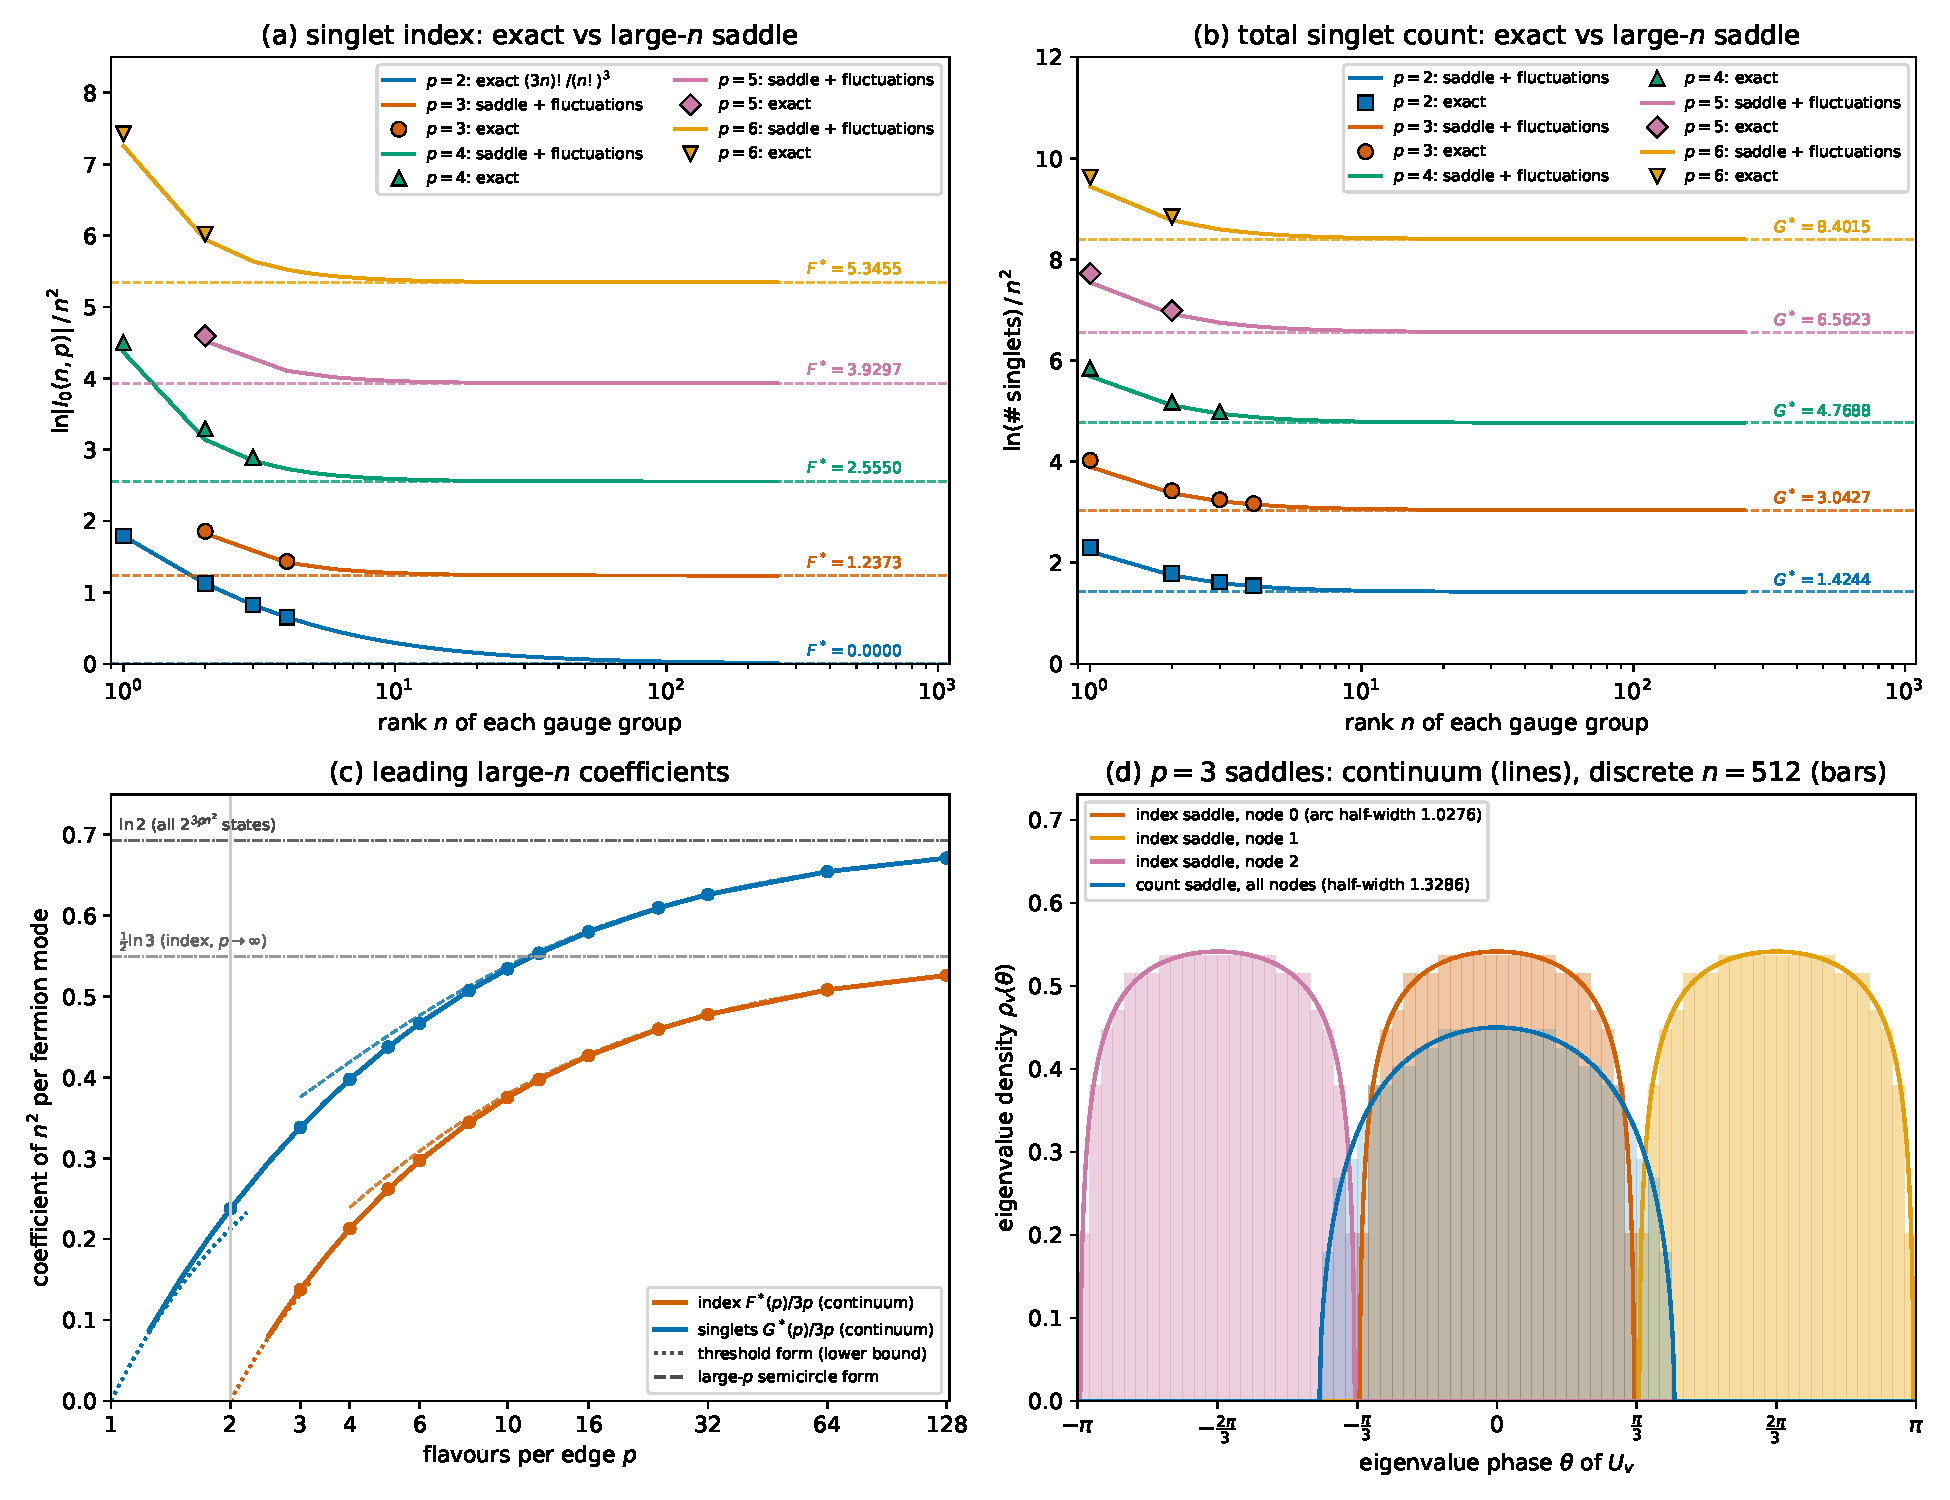
\includegraphics[width=0.98\textwidth]{report_figs/quiver_index_saddle.pdf}
\caption{The large-$n$ saddle. (a) $\ln|I_0|/n^2$ against $n$: exact values (markers), the saddle-point estimate with
Gaussian fluctuations and the universal crystal correction (lines), and the asymptotes $F^*(p)$ (dashed); for $p=2$
the line is the exact result \eqref{eq:p2}. (b) The same for the total singlet count. (c) The leading coefficients
per fermion mode against $p$, with the threshold bound and the large-$p$ asymptotics. (d) The equilibrium densities at
$p=3$: the three index arcs and the single arc of the count saddle, with histograms of the discrete maximum at
$n=512$.}
\label{fig:saddle}
\end{figure}

\subsection{\texorpdfstring{Finite $n$ and the test at $(4,3)$}{Finite n and the test at (4,3)}}

The coefficient $F^*$ alone cannot be compared with the data at $n\le4$: at $(4,3)$ it gives $F^*n^2=19.80$
against the exact $\ln|I_0|=22.97$, a factor of 24 too small. The subleading terms come from the same saddle. The
discrete maximum behaves as $L_{\max}=F^*n^2+3n\ln n+3n\int g\ln(2\pi g)+\frac14\ln n+O(1)$, where $g$ is the density of
one arc: the $n\ln n$ and $O(n)$ terms are the self-energy of each species at local spacing $1/(ng)$, which we
verified to six digits, and the $\frac14$ is consistent with $\frac1{24}$ per soft edge. Adding the Gaussian
fluctuations about the maximum overshoots by a universal amount, the excess of the harmonic approximation for a
$\beta=2$ log gas, which on the circle is $\ln(e/\sqrt{2\pi})$ per eigenvalue up to $O(1/n)$. With that correction the
estimate reproduces \eqref{eq:p2} to $1/36n$, and for $p\ne2$ we assume that each arc is locally a $\beta=2$ gas, which
is the one heuristic step. The resulting estimate has no free parameters, and Table~\ref{tab:laplace} compares it with
every non-zero exact value we have. All 27 residuals are negative and none exceeds $0.6$ in the logarithm, across
values from $e^{1.8}$ to $e^{50.7}$; at $(4,3)$ the estimate gives $22.69$, within $25\%$ of
$|I_0|=9.43\times10^9$. At large $n$ the $O(n)$ terms cancel to fit precision and the estimate takes the form
$\ln|I_0|\approx F^*n^2+\frac12\ln n+d(p)$, with $d\approx2.2$--$2.4$ for $p=3$--$6$, in line with the absence of an
$O(n)$ term in $\beta=2$ ensembles. For $p=3$ it predicts $\ln|I_0|\approx47.7$, $82.6$, $127.3$ and $181.8$ at
$n=6$, 8, 10 and 12, beyond the reach of the exact recursion.

\begin{table}[t]\centering\small
\begin{tabular}{ccccccc}
\toprule
& \multicolumn{3}{c}{$\ln|I_0|$} & \multicolumn{3}{c}{$\ln(\#\text{singlets})$}\\
\cmidrule(lr){2-4}\cmidrule(lr){5-7}
$(n,p)$ & exact & saddle & difference & exact & saddle & difference\\
\midrule
$(1,2)$ & 1.79 & 1.76 & $-0.03$ & 2.30 & 2.22 & $-0.08$ \\
$(2,2)$ & 4.50 & 4.49 & $-0.01$ & 7.15 & 7.00 & $-0.15$ \\
$(3,2)$ & 7.43 & 7.42 & $-0.01$ & 14.56 & 14.40 & $-0.17$ \\
$(4,2)$ & 10.45 & 10.45 & $-0.01$ & 24.75 & 24.55 & $-0.19$ \\
$(1,3)$ & \multicolumn{3}{c}{both vanish} & 4.03 & 3.90 & $-0.13$ \\
$(2,3)$ & 7.43 & 7.30 & $-0.12$ & 13.70 & 13.50 & $-0.20$ \\
$(3,3)$ & \multicolumn{3}{c}{both vanish} & 29.22 & 28.97 & $-0.25$ \\
$(4,3)$ & 22.97 & 22.69 & $-0.28$ & 50.74 & 50.44 & $-0.30$ \\
$(1,4)$ & 4.50 & 4.37 & $-0.13$ & 5.85 & 5.69 & $-0.16$ \\
$(2,4)$ & 13.16 & 12.56 & $-0.60$ & 20.69 & 20.45 & $-0.24$ \\
$(3,4)$ & 26.02 & 25.62 & $-0.39$ & 44.85 & 44.54 & $-0.30$ \\
$(1,5)$ & \multicolumn{3}{c}{both vanish} & 7.72 & 7.54 & $-0.18$ \\
$(2,5)$ & 18.38 & 18.08 & $-0.29$ & 27.94 & 27.68 & $-0.26$ \\
$(1,6)$ & 7.43 & 7.26 & $-0.17$ & 9.63 & 9.44 & $-0.19$ \\
$(2,6)$ & 24.08 & 23.78 & $-0.30$ & 35.37 & 35.09 & $-0.28$ \\
\bottomrule
\end{tabular}
\caption{The saddle-point estimate (Gaussian fluctuations about the discrete saddle, minus the universal $\beta=2$
crystal excess, no free parameters) against all exact values. For odd $p$ and odd $n$ the index and the estimate
both vanish exactly, the latter because the two orientations of the arcs cancel.}
\label{tab:laplace}
\end{table}

The status of these statements should be clear. The rewriting \eqref{eq:loggas}, the formula \eqref{eq:p2} and the
sign rules are exact. The coefficient $F^*$ for even $p$ rests on standard large-deviation results for log gases,
which we have not reproved. For odd $p$ it also requires that the sign $\sigma^p$ does not cancel the leading saddle.
Sign changes need an eigenvalue of one node to pass an eigenvalue of a neighbouring node across the gap between arcs,
which costs an action of order $n$; but the gap at $p=3$ is only $0.039$ radians, so the suppression is modest at the
sizes of interest. The exact values at $(2,3)$ and $(4,3)$ show no sign of cancellation, their residuals being like
those at even $p$. Finally, $|I_0|$ is a lower bound on the number of singlet BPS states, equal to it only in the
absence of cancellations between degrees, for example under concentration; and for odd $pn^2$ the index vanishes and
says nothing about that number.

\section{\texorpdfstring{Prospects for the $p\ge3$ quiver}{Prospects for the p>=3 quiver}}\label{sec:prospects}

Table~\ref{tab:scorecard} sets the two cases side by side. The contrast is sharp. The $p=2$ quiver is an elegant and highly
structured corner, with a hidden $\mathcal N=4$ on singlets, an exact index and a spectrum that is not random-matrix
like, but its BPS entropy is provably sub-macroscopic. The $p\ge3$ quiver has every property we have been able to
test at the level we would hope for: a singlet BPS entropy that is a finite fraction of the total at order $n^2$, a
concentrated BPS sector, chaotic non-BPS spectra, small gaps next to the BPS degree, and only $\mathcal N=2$
supersymmetry, which is what the $\mathcal N=2$ super-Schwarzian needs. The large-$p$ limit adds a pleasing
interpolation: the singlet BPS entropy per fermion rises from zero at $p=2$ towards the SYK value at $p=\infty$,
so the flavour number dials between a gauge-dominated matrix regime and an SYK-like one, with planar large-$n$
control at every $p$.

\begin{table}[t]\centering\small
\begin{tabular}{p{0.19\textwidth}p{0.33\textwidth}p{0.39\textwidth}}
\toprule
property & $p=2$ & $p=3$ (and $p\ge3$)\\
\midrule
BPS entropy & $\ln|I_0|=3n\ln3+O(\ln n)$, proved; not macroscopic &
$\ln|I_0|=F^*(p)n^2+O(\ln n)$, $F^*(3)=1.2373$, $41\%$ of the singlet log-count (large-deviation level; sign proviso
for odd $p$)\\
Concentration & $(2,2)$: all 90 singlet BPS states at $k=12$, exact & $(2,3)$: all 1680 at $k=18$, numerical;
$n\ge3$ open; index signs consistent\\
Fortuity & $(2,2)$: all 90 classes obstructed at first order & untested; follows from concentration at the next rank\\
Non-BPS statistics & not random-matrix; hidden $\mathcal N=4$ on singlets & Gaussian orthogonal, $10\,024$ levels at
$(2,3)$\\
Near-BPS gap & none ($\ge95.6$) & $0.054$ next to the BPS degree; Turiaci--Witten not yet testable\\
Supersymmetry & $\mathcal N=4$ on singlets (numerical, $n=2$) & $\mathcal N=2$\\
Large $n$ & planar; exact index & planar; index saddle solved\\
\bottomrule
\end{tabular}
\caption{Desirable properties of the quiver for $p=2$ and $p\ge3$, with their status.}
\label{tab:scorecard}
\end{table}

The caveats are equally clear, and they define the programme. Almost everything except the entropy has been
established at $n=2$ only, and concentration is the property most at risk as $n$ grows: in the adjoint models it was
the growth of the window with the rank that failed, and although its mechanism is absent here, nothing yet proves that
another one does not take its place. The near-BPS gaps at $(2,3)$ are suggestive, but at this size the neighbouring
charge sectors differ too much in entropy for the Turiaci--Witten density to apply, so the super-Schwarzian
question remains open. Fortuity at $p\ge3$ is untested, although it would follow from concentration at the next rank and there is no reason to expect a different answer
from $(2,2)$. And the model is planar rather than melonic, so at fixed $p$ there is no analogue of the SYK Schwinger--Dyson
solution; large-$n$ dynamics has to come from the bootstrap, from other matrix-model methods, or from the large-$p$
limit discussed below.

Several next steps follow, and the first observation is that concentration beyond $n=2$ has to be settled without
help from the index. Since $Q$ raises the fermion number by three and every singlet has $k\equiv0$ mod 3, no
R-charge fugacity is compatible with the pairing of non-BPS states in the singlet sector: $\Tr(-1)^ky^{k/3}$ is
protected only at $y=1$. The singlet index is therefore the only protected quantity of the gauged model, and its
sign, which always agrees with half filling, is all it can say about where the BPS states sit.

The exact methods reach exactly one more point. With a singlet-adapted basis, built from the dual-Cauchy components
with $Q$ acting as Pieri maps, the singlet spaces at $(3,2)$ have $3\,494$ states at $k=12$ and $558\,304$ at half
filling, so concentration, the near-BPS gap and the multiplet statistics can be followed from $n=2$ to $n=3$, albeit
in the $p=2$ corner. The same basis at $(2,3)$, $300\,584$ singlets at half filling, yields the 1680 BPS vectors for a
direct test of BPS chaos and of fortuity at $p=3$. Beyond that the singlet sectors explode: at $(3,3)$ they hold
$1.2\times10^8$ states at $k=18$ and $1.1\times10^{12}$ at half filling, and $3\times10^8$ at half filling at $(2,4)$.

At $p=3$ and $n\ge3$ the matrix bootstrap \cite{HHK,LZ,LM}, which we developed in sector-resolved form for the
adjoint models \cite{R2}, must take over, and its natural first targets are certificates of absence. A positive
lower bound on the singlet energy at $(3,3)$ and $k=18$, far from the window where such certificates are easiest,
would prove that all 1680 classes at $(2,3)$ are fortuitous; certificates for $k\le36$ would confine the BPS states at
$(3,3)$ to the two singlet degrees adjacent to half filling, which is concentration at the first rank beyond exact
methods. The near-BPS gaps and their scaling with $n$, the actual super-Schwarzian test, are the harder final target.

On the analytic side, the large-$p$ limit is where the model should become SYK-like. The holonomy saddle realises
precisely the $\mathbb Z_3$ twist that makes the index of $\mathcal N=2$ SYK large, and at fixed $n$ the $3pn^2$
fermions with random flavour couplings should be governed by the Schwinger--Dyson equations of \cite{FGMS}, with a
gauge correction of relative order $1/p$ since $\dim G/\dim V=1/p$. Deriving the super-Schwarzian and the chaos
exponent in this limit, and reproducing the exact large-$p$ expansion of $F^*(p)$ in Table~\ref{tab:saddle} as a
check, would establish the desired dynamics in a controlled corner of the same model; that $F^*(p)$ is smooth for all
$p>2$ suggests that $p=3$ lies in the same phase. Monte Carlo integration of \eqref{eq:loggas}, by thermodynamic
integration in $p$ from the exact point $p=2$, would test the finite-$n$ predictions at $n=6$--12, and the generalised
monotones of \cite{CCK} should be checked. Finally, the hidden $\mathcal N=4$ of the $p=2$ quiver deserves a
derivation and a test at $n=3$, both for its own sake and because a small $\mathcal N=4$ super-Schwarzian would require
an $SU(2)$ R-symmetry that we have not found.

In summary, the fermionic $U(n)^3$ quiver with $p\ge3$ flavours is, to our knowledge, a new candidate for a matrix
SYK model. It has macroscopic and, at the sizes we can reach, concentrated BPS entropy, chaotic multiplet spectra and
near-BPS gaps; it reduces to an exactly solvable log gas at the level of the index; and its large-$p$ limit makes contact
with $\mathcal N=2$ SYK. Whether concentration survives at large $n$ is now the central question; the singlet-adapted
computation at $(3,2)$, bootstrap certificates at $(3,3)$ and the large-$p$ limit are the next steps.

\appendix
\section{Methods and reproducibility}\label{app:methods}

All computations are reproducible from the repository, with the parameters, seeds, outputs and memory use recorded
in the result files. Cohomology at $(2,2)$ uses exact ranks modulo primes. The $n=2$ spectra use Weyl-reduced
zero-weight sectors (\path{src/quiver_n2.py}) with the exact Casimir penalty, Lanczos (\path{scripts/quiver_singlet_zero_modes.py}),
dense singlet bases (\path{scripts/quiver_singlet_spectrum.py}), the Casimir-polynomial projection for the
$10\,024$-level pair (\path{scripts/quiver_singlet_pair_large.py}, float64, peak 8.6~GB) and the
$\mathcal N=4$ and symmetry analysis (\path{scripts/quiver_p2_n4.py}, \path{scripts/quiver_commutant.py}).
The fortuity test is \path{scripts/run_quiver_fortuity.py}. Singlet indices use \path{src/quiver_index.py}
(dual Cauchy and the Littlewood--Richardson transfer matrix, exact integers). The log-gas analysis is
\path{src/quiver_saddle.py} and \path{scripts/quiver_index_saddle.py}, tested by \path{tests/test_quiver_saddle.py}
(reduced against full energies, Hessians against finite differences to $10^{-10}$, the $p=2$ formula, the continuum
values, and the eigenvalue representation against direct quadrature at $n=1$). The derivations are written out in
\path{docs/derivations.md} (D18) and the research log in \path{research/notes/quiver_project.md}. The main data
files are \path{results/data/quiver_singlet_index_dixon.json}, \path{quiver_singlet_zero_modes_n2_p3_k*.json},
\path{quiver_singlet_pair_n2_p3_k9_f64.json}, \path{quiver_p2_n4_*.json}, \path{quiver_fortuity_n2_p2_k12.json} and
\path{quiver_index_saddle.json}.

\begin{thebibliography}{99}\small
\bibitem{ChangLin} C.-M.~Chang and Y.-H.~Lin, \emph{Holographic covering and the fortuity of black holes},
arXiv:2402.10129.
\bibitem{CCSY} C.-M.~Chang, Y.~Chen, B.~S.~Sia and Z.~Yang, \emph{Fortuity in SYK models}, JHEP \textbf{08} (2025)
003, arXiv:2412.06902.
\bibitem{FGMS} W.~Fu, D.~Gaiotto, J.~Maldacena and S.~Sachdev, \emph{Supersymmetric Sachdev--Ye--Kitaev models},
Phys.\ Rev.\ D \textbf{95} (2017) 026009, arXiv:1610.08917.
\bibitem{TW} G.~J.~Turiaci and E.~Witten, \emph{$\mathcal N=2$ JT supergravity and matrix models},
arXiv:2305.19438.
\bibitem{Chen} Y.~Chen, \emph{Fortuity with a single matrix}, arXiv:2511.00790.
\bibitem{R1} Project report, \emph{Fermionic matrix models, fortuity, and SYK}, September 2026
(\path{research/pdfs/gauge_concentration_report.pdf}).
\bibitem{R2} Project report, \emph{Fermionic matrix models, fortuity, and the bootstrap}, October 2026
(\path{research/pdfs/matrix_fortuity_bootstrap_report.pdf}).
\bibitem{Witten} E.~Witten, \emph{An SYK-like model without disorder}, arXiv:1610.09758.
\bibitem{PSV} C.~Peng, M.~Spradlin and A.~Volovich, \emph{A supersymmetric SYK-like tensor model}, JHEP \textbf{05}
(2017) 062, arXiv:1612.03851.
\bibitem{CCR} C.-M.~Chang, S.~Colin-Ellerin and M.~Rangamani, \emph{On melonic supertensor models}, JHEP \textbf{10}
(2018) 157, arXiv:1806.09903.
\bibitem{BLM} A.~Biggs, L.~L.~Lin and J.~Maldacena, \emph{A melonic quantum mechanical model without disorder},
arXiv:2601.08908.
\bibitem{Bena} I.~Bena, M.~Berkooz, J.~de~Boer, S.~El-Showk and D.~Van~den~Bleeken, \emph{Scaling BPS solutions and
pure-Higgs states}, JHEP \textbf{11} (2012) 171, arXiv:1205.5023.
\bibitem{Tierz} M.~Tierz, \emph{BPS spectra of $\Tr[\Psi^p]$ matrix models for odd $p$}, arXiv:2604.27164.
\bibitem{CCK} J.~Choi, S.~Choi and S.~Kim, \emph{Fortuity on the conifold}, arXiv:2609.19297.
\bibitem{HHK} X.~Han, S.~A.~Hartnoll and J.~Kruthoff, \emph{Bootstrapping matrix quantum mechanics}, Phys.\ Rev.\
Lett.\ \textbf{125} (2020) 041601, arXiv:2004.10212.
\bibitem{LZ} H.~W.~Lin and Z.~Zheng, \emph{High-precision bootstrap of multimatrix quantum mechanics},
arXiv:2507.21007.
\bibitem{LM} S.~Laliberte and B.~McPeak, \emph{Bootstrapping supersymmetric (matrix) quantum mechanics},
arXiv:2510.01356.
\bibitem{AMMPV} O.~Aharony, J.~Marsano, S.~Minwalla, K.~Papadodimas and M.~Van~Raamsdonk, \emph{The
Hagedorn/deconfinement phase transition in weakly coupled large $N$ gauge theories}, Adv.\ Theor.\ Math.\ Phys.\
\textbf{8} (2004) 603, hep-th/0310285.
\end{thebibliography}

\end{document}
